%!TEX root=kdd15_workshop_main.tex
\section{Methodology} \label{sec:meth}
While there are many possible heuristics for streaming partitioning~\cite{Stanton:2012:SGP:2339530.2339722}, the most effective by far have been \emph{weighted, greedy} approaches. We maintain a compressed array storing the partition assignments of vertices streamed so far ($P_i^t$ for each process $i$ at time $t$). As each vertex $v$ is streamed, we count the edges from that vertex to each partition $|P_i^t \cap N(v)|$. This intuitively maximizes \emph{modularity}, the ratio of intra-partition edges to inter-partition edges. However, using this value on its own would result in all vertices being assigned to a single, large partition. Thus, we exponentially \emph{weight} the edge counts by the size of partitions $|P_i^t|$, relatively dampening the scores for partitions that are too large (but penalizing only lightly for small differences in size). This gives us two parameters: the linear importance of partition size to the score, $\alpha$, and the exponential rate at which increasing partition size incurs a greater penalty, $\gamma$. This yields the basic `FENNEL' algorithm~\cite{tsourakakis2012fennel} shown in~\RefAlgorithm{alg:fennel}.

\begin{algorithm}
 Set all $P_i$ to $\emptyset$\;
 \ForEach{$v \in V(G)$ as it arrives at time $t$}{
   $j \gets \displaystyle \argmax_{i\in\{1,\dots,p\}}|P_i^t \cap N(v)| - \alpha \frac{\gamma}{2}|P_i^t|^{\gamma-1}$\;
   Add $v$ to set $P_j^{t+1}$\;
 }
 \caption{Serial streaming FENNEL partitioner}
 \label{alg:fennel}
\end{algorithm}

Exact computation of this algorithm as described is not possible in parallel, because $P_i^{t-1}$ must be known to compute $P_i^t$. A multi-threaded approximation of this algorithm is easily performed by relaxing this requirement and using $P_i^{t-p}$ to compute $P_i^t$, where $p$ is the number of threads. This resulted in only a small drop in partition quality in our experiments: the serial algorithm is already inherently approximate, and $p$ is very small compared to $|V|$.

To compute this algorithm in distributed memory, a naive approach is to constantly broadcast and apply partition assignments as they are computed. Without synchronization, this results in a drastic drop in partition quality, because the latency across a network is high enough that partition assignments are perpetually out of date. Synchronization, if implemented efficiently, could be used to improve partition quality of a single pass at the expense of poorer scalability. However, we instead emphasize an approach that achieves even higher partition quality and balance through \emph{multiple} streams with minimal synchronization.

Our implementation follows the methodology of `restreaming partitioning'~\cite{nishimura2013restream}, which shows the single-pass algorithms of FENNEL and WDG~\cite{tsourakakis2012fennel,Stanton:2012:SGP:2339530.2339722} can be repeated over the same data in the same order, yielding a convergent improvement in quality. This approach has other benefits that we utilize:

\begin{itemize}
\item Partition data is only communicated between streams, yielding high parallelism.
\item Parameters ($\alpha, \gamma)$ can be `tempered' to achieve higher-quality, balanced results that avoid immediate global minima.
\end{itemize}

\subsection{\ourmethod}
\ourmethod operates on a distributed graph $G$ in distributed CSR format. We take as input the parameters $\alpha, \gamma$, the number of partitions \numprocsparm (assumed to be equal to the number of MPI processes), the number of re-streams $\numrestreamsparm$, and the `tempering' parameter \expparm. \ourmethod then performs $\numrestreamsparm$ iterative passes over the graph (in identical random order), multiplicatively increasing the balance parameter by \expparm with each pass. This promotes a high-quality, but less-balanced partition early on, while further promoting balance with each subsequent pass~\cite{nishimura2013restream}. 

Between each pass, the partition information (an array that maps each vertex to a partition) is communicated across all processors using the MPI \textsc{AllGather} primitive, which is often optimized for a given network architecture. The pseudocode for \ourmethod is shown in~\RefAlgorithm{alg:grasp}. Here, $P_{i,p}^{t}$ is the $i$th partition set maintained on process $p$ at time $t$.

\begin{algorithm}
\ForPar{each process $p$}{
	$vorder \gets rand\_perm(\{0,\dots,|V(G_{local})|\})$\;
	Randomly assign local vertices to partitions $P_{i,p}^0$\;
}
\For{$run \gets \{ 1 \dots \numrestreamsparm \}$} {
	\ForPar{each process $p$}{
		\ForEach{$v \in vorder$}{
			$j \gets \displaystyle \argmax_{i\in\{1,\dots,p\}}|P_{i}^t \cap N(v)| - \alpha \frac{\gamma}{2}|P_{i}^t|^{\gamma-1}$\;
			Add $v$ to set $P_{j,p}^{t+1}$\;
		}
	}
	\textsc{MPI\_AllGather} global partition assignments\;
	$\alpha \gets \expparm \alpha$ 
}
 \caption{Parallel Restreaming performed by \ourmethod.}
 \label{alg:grasp}
\end{algorithm}

This method is illustrated graphically in~\RefFigure{fig:restream}. In practice, we store the partitioning in a single compressed array, updating partition assignments in-place while storing a running count of the partition sizes. 

To increase accuracy, we found it necessary to update the global partition sizes $|P_{i}^t|$ at finer granularities within the stream. Since there are only $p$ such values, this incurs a very small amount of communication. In our experiments we used the \textsc{MPI\_AllReduce} primitive to update partition sizes every time we had processed a constant number of vertices. We found that updating every 4096 vertices yielded good quality with only a small performance hit. This is a natural target to optimize with non-blocking primitives.

\begin{figure}[ht]
\centering
  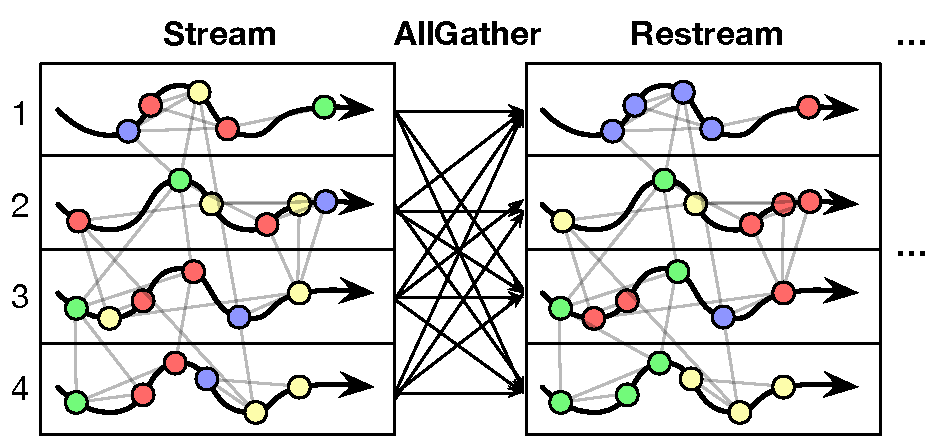
\includegraphics[width=1.0\columnwidth]{figures/restreamdiagram.pdf}
  %\caption{Partition speed of various Kronecker graphs.}
  \caption{Two parallel restreaming steps on four processes.}
  \label{fig:restream}
\end{figure}


In~\RefAlgorithm{alg:grasp}, each process computes $\bigO{\numrestreamsparm \cdot \frac{|E|+|V|}{p}}$ work, and the network incurs a time of $\numrestreamsparm \cdot T_{allgather}(|V(G)|)$. $\numrestreamsparm$ is determined by restreaming until some criteria is satisfied (either that we have encountered a local minimum, or we have achieved a good tradeoff between balance and edge-cut), or by choosing a number of restreamings and setting the tempering parameter $\expparm$ so that we achieve perfect balance within that number. In our experiments, we generally see good partitions within 10 restreams. 
